\subsubsection{UC6 - Gestione Carrello}
 \begin{figure}[h]
	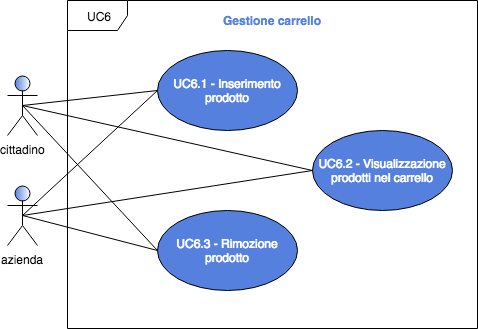
\includegraphics[width=9cm]{res/images/UC6GestioneCarrello.png}
	\centering
	\caption{UC6 - Gestione carrello}
\end{figure}
\begin{itemize}
	\item \textbf{Attori Primari}: cittadino, azienda\glo;
	\item \textbf{Descrizione}: l'utente, che sia esso cittadino o azienda, ha il totale controllo del proprio carrello, con possibilità di aggiunta e rimozione di prodotti e/o servizi, con possibilità di trarne un riepilogo;
	\item \textbf{Scenario}: l'utente in questione intende comprare un bene e/o un servizio:
	 \begin{enumerate}[label=\alph*.]
		\item inserimento prodotto [UC6.1];
		\item visualizzazione prodotti nel carrello [UC6.2];
		\item rimozione prodotto [UC6.3];
	\end{enumerate}
	\item \textbf{Precondizione}: l'utente necessita di acquistare un prodotto o un servizio;
	\item \textbf{Postcondizione}: l'utente può procedere all'acquisto di tutti i beni e/o servizi presenti nel carrello.
\end{itemize} 
 \subsubsection{UC6.1 - Inserimento prodotto}
\begin{itemize}
	\item \textbf{Attori Primari}: cittadino, azienda\glo;
	\item \textbf{Descrizione}: l'utente inserisce il prodotto selezionato all'interno del proprio carrello;
	\item \textbf{Scenario}: l'utente si trova all'interno della pagina di un bene o servizio e clicca sul pulsante dedicato all'aggiunta dello stesso nel carrello virtuale;
	\item \textbf{Precondizione}: l'utente deve essere all'interno della pagina di un bene o un servizio;
	\item \textbf{Postcondizione}: nel carrello dell'utente è presente il bene o il servizio in quantità definite dall'utente stesso nella fase di visualizzazione della pagina del bene o del servizio in questione [UC5].
\end{itemize}
 \subsubsection{UC6.2 - Visualizzazione prodotti del carrello}
  \begin{figure}[h]
 	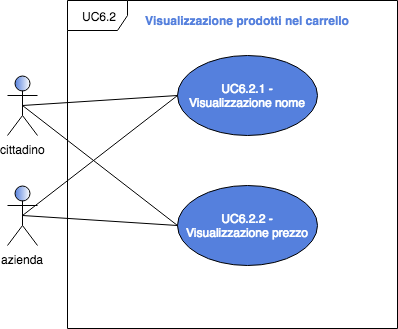
\includegraphics[width=7cm]{res/images/UC6-2VisualizzazioneProdottiCarrello.png}
 	\centering
 	\caption{UC6.2 - Visualizzazione prodotti del carrello}
 \end{figure}
\begin{itemize}
	\item \textbf{Attori Primari}: cittadino, azienda\glo;
	\item \textbf{Descrizione}: l'utente visualizza un riepilogo di tutti i prodotti presenti all'interno el proprio carrello;
	\item \textbf{Scenario}: l'utente si trova all'interno della pagina del proprio carrello virtuale e può apprezzare una lista di prodotti se essi sono stati aggiunti al carrello, in particolare per ognino di essi può trarre le informazioni:
	 \begin{enumerate}[label=\alph*.]
		\item visualizzazione nome [UC6.2.1];
		\item visualizzazione prezzo [UC6.2.2];
	\end{enumerate} 
	\item \textbf{Precondizione}: l'utente deve essere all'interno della pagina ddel proprio carrello;
	\item \textbf{Postcondizione}: l'utente è consapevole di tutti i prodotti all'interno del proprio carrello.
\end{itemize}
 \subsubsection{UC6.2.1 - Visualizzazione nome}
\begin{itemize}
	\item \textbf{Attori Primari}: cittadino, azienda\glo;
	\item \textbf{Descrizione}: l'utente visualizza il nome del bene o del servizio presente nel carrello;
	\item \textbf{Scenario}: l'utente si trova all'interno della pagina del proprio carrello;
	\item \textbf{Precondizione}: l'utente deve aver inserito almeno un bene o un servizio nel proprio carrello;
	\item \textbf{Postcondizione}: l'utente conosce il nome del prodotto presente nel carrello.
\end{itemize}
 \subsubsection{UC6.2.2 - Visualizzazione prezzo}
\begin{itemize}
	\item \textbf{Attori Primari}: cittadino, azienda\glo;
	\item \textbf{Descrizione}: l'utente visualizza il prezzo del bene o del servizio presente nel carrello;
	\item \textbf{Scenario}: l'utente si trova all'interno della pagina del proprio carrello;
	\item \textbf{Precondizione}: l'utente deve aver inserito almeno un bene o un servizio nel proprio carrello;
	\item \textbf{Postcondizione}: l'utente conosce il prezzo del prodotto presente nel carrello.
\end{itemize}
 \subsubsection{UC6.3 - Rimozione prodotto}
\begin{itemize}
	\item \textbf{Attori Primari}: cittadino, azienda\glo;
	\item \textbf{Descrizione}: l'utente rimuove il prodotto selezionato dal proprio carrello;
	\item \textbf{Scenario}: l'utente si trova all'interno del carrello e clicca sul pulsante dedicato alla rimozione dello stesso dal carrello virtuale;
	\item \textbf{Precondizione}: l'utente deve essere all'interno della pagina del proprio carrello;
	\item \textbf{Postcondizione}: nel carrello dell'utente non vi è più presente il bene o il servizio rimosso.
\end{itemize}